%%%%%
%%
%% Sample document ``thesis.tex''
%%
%% Version: v0.2
%% Authors: Jean Martina, Rok Strnisa, Matej Urbas
%% Date: 30/07/2008
%%
%% Copyright (c) 2008-2011, Rok Strniša, Jean Martina, Matej Urbas
%% License: Simplified BSD License
%% License file: ./License
%% Original License URL: http://www.freebsd.org/copyright/freebsd-license.html
%%%%%

% Available documentclass options:
%
%   <all `report` document class options, e.g.: `a5paper`>
%   withindex   - enables the index. New index entries can be added through `\index{my entry}`
%   glossary    - enables the glossary.
%   techreport  - typesets the thesis in the technical report format.
%   firstyr     - formats the document as a first-year report.
%   times       - uses the `Times` font.
%   backrefs    - add back references in the Bibliography section
%
% For more info see `README.md`
\documentclass[withindex,glossary]{cam-thesis}
\addtocontents{toc}{\protect\setcounter{tocdepth}{1}}
\setcounter{secnumdepth}{2}

% Citations using numbers
\usepackage[numbers]{natbib}

\usepackage{tikz}
\usetikzlibrary{calc,tikzmark,decorations.pathmorphing}
\usetikzlibrary{arrows.meta}
\usetikzlibrary{shapes,shapes.geometric,graphs,quotes,arrows.meta,positioning,calc,chains,trees}
\usetikzlibrary{decorations,trees,spy,shadows,backgrounds,fit,trees,matrix,automata}
\usetikzlibrary{shadows.blur}
\usetikzlibrary{tikzmark}
\usetikzlibrary{fit}
\usetikzlibrary{chains}
\usetikzlibrary{decorations.pathreplacing,arrows.meta,calc,positioning,calligraphy}

\usepackage{pgfplots}
\pgfplotsset{compat=1.18}
\usepgfplotslibrary{statistics}

\usepackage{minted}

\usepackage[T1]{fontenc}
\usepackage[scaled=0.8]{beramono}

\usepackage{listings}
\usepackage{booktabs}
\usepackage[inline]{enumitem}


% https://tex.stackexchange.com/questions/30504/how-can-i-properly-align-the-line-numbers-of-a-source-code-listing-with-the-marg

\newlength{\MaxSizeOfLineNumbers}%
\settowidth{\MaxSizeOfLineNumbers}{99}% Adjust to maximum number of lines
\addtolength{\MaxSizeOfLineNumbers}{2ex}%

\lstdefinestyle{scriptStyle}{%
  basicstyle=\ttfamily\lst@ifdisplaystyle\scriptsize\fi,
  keywordstyle=\ttfamily\lst@ifdisplaystyle\color{brown}\scriptsize\fi,
  commentstyle=\ttfamily\lst@ifdisplaystyle\color{commentcolour}\scriptsize\fi,
}

% \lstset{
%   % aboveskip=0pt,
%   % belowskip=0pt,
%   % xleftmargin=0pt,
%   % framesep=0pt,
%   basicstyle=\ttfamily,%\lst@ifdisplaystyle\scriptsize\fi,
%   keywordstyle=\ttfamily,%\lst@ifdisplaystyle\color{brown}\scriptsize\fi,
%   commentstyle=\ttfamily,%\lst@ifdisplaystyle\color{blue}\scriptsize\fi,
%   % morecomment=[s][\color{blue}]{/*@}{@*/},
%   % xleftmargin=5.0ex,
%   % numberstyle=\tiny,
%   % framexleftmargin=1em
% }

\definecolor{commentcolour}{RGB}{0,100,0}

\lstset{
%  aboveskip=0pt,
%  belowskip=0pt,
   xleftmargin=5mm,
%  framesep=0pt,
  basicstyle=\ttfamily\small,
  keywordstyle=\ttfamily\bfseries\color{black},
  commentstyle=\ttfamily\color{commentcolour},
%%   keywordstyle=\ttfamily\lst@ifdisplaystyle\bfseries\scriptsize\fi,
%%   commentstyle=\ttfamily\lst@ifdisplaystyle\itshape\scriptsize\fi,
  % morecomment=[s][\color{blue}]{/*@}{@*/},
  % xleftmargin=5.0ex,
  numbers=left,
  numberstyle=\tiny,
  % framexleftmargin=1em
  escapeinside={!}{!},
  showstringspaces=false,
}

\lstset{language=C}




%%%%%%%%%%%% listings for CN, from Iris slides

\lstdefinelanguage{CNC}{%
  language     = C,
  morekeywords={
    Owned,
    Block,
    integer,
    pointer, 
    predicate, 
    let, 
    each, 
    assert, 
    instantiate, 
    pack, 
    unpack,
    list,
    function,
    take,
    tuple,
    datatype,
    requires,
    ensures
  },
}


%%%%%%%%%%%%%%%%%%%%%%%%%%%%%%%%%%%%%%%%%%%%%%%%%%%%%%%%%%%%%%%%%%%%%%%%%%%%%%%%
%% Thesis meta-information
%%

%% The title of the thesis:
\title{Executable separation-logic\\
specifications}

%% The full name of the author (e.g.: James Smith):
\author{Rini Banerjee}

%% College affiliation:
\college{Newnham College}

%% College shield [optional]:
% \collegeshield{CollegeShields/Christs}
% \collegeshield{CollegeShields/Churchill}
% \collegeshield{CollegeShields/Clare}
% \collegeshield{CollegeShields/ClareHall}
% \collegeshield{CollegeShields/CorpusChristi}
% \collegeshield{CollegeShields/Darwin}
% \collegeshield{CollegeShields/Downing}
% \collegeshield{CollegeShields/Emmanuel}
% \collegeshield{CollegeShields/Fitzwilliam}
% \collegeshield{CollegeShields/Girton}
% \collegeshield{CollegeShields/GonCaius}
% \collegeshield{CollegeShields/Homerton}
% \collegeshield{CollegeShields/HughesHall}
% \collegeshield{CollegeShields/Jesus}
% \collegeshield{CollegeShields/Kings}
% \collegeshield{CollegeShields/LucyCavendish}
% \collegeshield{CollegeShields/Magdalene}
% \collegeshield{CollegeShields/MurrayEdwards}
\collegeshield{CollegeShields/Newnham}
% \collegeshield{CollegeShields/Pembroke}
% \collegeshield{CollegeShields/Peterhouse}
% \collegeshield{CollegeShields/Queens}
% \collegeshield{CollegeShields/Robinson}
% \collegeshield{CollegeShields/Selwyn}
% \collegeshield{CollegeShields/SidneySussex}
% \collegeshield{CollegeShields/StCatharines}
% \collegeshield{CollegeShields/StEdmunds}
% \collegeshield{CollegeShields/StJohns}
% \collegeshield{CollegeShields/Trinity}
% \collegeshield{CollegeShields/TrinityHall}
% \collegeshield{CollegeShields/Wolfson}
% \collegeshield{CollegeShields/CUniNoText}
% \collegeshield{CollegeShields/FitzwilliamRed}

%% Submission date [optional]:
% \submissiondate{November, 2042}

%% You can redefine the submission notice [optional]:
% \submissionnotice{A badass thesis submitted on time for the Degree of PhD}

%% Declaration date:
\date{My Month, My Year}

%% PDF meta-info:
\subjectline{Computer Science}
\keywords{one two three}



%%%%%%%%%%%%%%%%%%%%%%%%%%%%%%%%%%%%%%%%%%%%%%%%%%%%%%%%%%%%%%%%%%%%%%%%%%%%%%%%
%% Abstract:
%%
\abstract{%
  My abstract ...
}



%%%%%%%%%%%%%%%%%%%%%%%%%%%%%%%%%%%%%%%%%%%%%%%%%%%%%%%%%%%%%%%%%%%%%%%%%%%%%%%%
%% Acknowledgements:
%%
\acknowledgements{%
My acknowledgements\ldots
  % I would like to start by thanking my supervisors, Peter Sewell and Neel Krishnaswami. When I first received my PhD offer to work with them, someone described them to me as two giants of our field. I believe that description to be wholly accurate, and yet every day since I came to Cambridge, these two giants (physically, and metaphorically) have graciously met me at my level, providing support, guidance, humour, understanding, and much more than I can express. Thank you to Peter for teaching me how to persevere in the face of uncertainty (i.e.~bash my head against the wall), and the importance of scientific rigour, and that even very simple ideas can be very useful and should not be automatically dismissed. Thank you to Neel for being an encyclopaedia of knowledge and PL literature, to whom no question was ever too simple, and for exposing me to various streams of more theoretical research during my PhD. Thank you to both for teaching me how to communicate my research to other people, and emphasising its importance.
}

% My maternal grandfather, who was an engineer and general manager of a steel plant in Bengal; and my paternal grandmother, who did not receive a formal education beyond primary school; who also happen to be two people renowned for their kindness towards others.

% Peter and Neel
% Kayvan. Christopher, Dhruv, Hiro, David
% Lise + Cambridge Trust
% Saljuk
% Waterstone's, Harvey's
% Parents


%%%%%%%%%%%%%%%%%%%%%%%%%%%%%%%%%%%%%%%%%%%%%%%%%%%%%%%%%%%%%%%%%%%%%%%%%%%%%%%%
%% Glossary [optional]:
%%
\newglossaryentry{HOL}{
    name=HOL,
    description={Higher-order logic}
}

\newif\ifclean
\cleantrue
% \cleanfalse

\ifclean
\newcommand\TODO[1]{}
\else
\newcommand\TODO[1]{{\color{violet}TODO: #1}}
\fi


%%%%%%%%%%%%%%%%%%%%%%%%%%%%%%%%%%%%%%%%%%%%%%%%%%%%%%%%%%%%%%%%%%%%%%%%%%%%%%%%
%% Contents:
%%
\begin{document}



%%%%%%%%%%%%%%%%%%%%%%%%%%%%%%%%%%%%%%%%%%%%%%%%%%%%%%%%%%%%%%%%%%%%%%%%%%%%%%%%
%% Title page, abstract, declaration etc.:
%% -    the title page (is automatically omitted in the technical report mode).
\frontmatter{}




%%%%%%%%%%%%%%%%%%%%%%%%%%%%%%%%%%%%%%%%%%%%%%%%%%%%%%%%%%%%%%%%%%%%%%%%%%%%%%%%
%% Thesis body:
%%
% \chapter{[To delete] Outline}

% \begin{enumerate}
%   \item Introduction
%   \item Background + related work
%   \item Motivating example, including partial + fragmentary specifications
%   \begin{enumerate}
%     \item Meld previous simpler CN spec example with narrative from PLDI submission overview section
%   \end{enumerate}
%   \item Formalisation (Dhruv) -- incl. unpublished partial spec formalisation by Hiro?
%   \begin{enumerate}
%     \item Formalisation of Fulminate's dynamic ownership tracking scheme
%     \item Relationship between that and explicit resource passing scheme
%   \end{enumerate}
%   \item Implementation
%   \begin{enumerate}
%     \item Architecture (incl. diagram from Fulm paper, or something similar). Has diverged a bit now as CN and Fulm wf checks are slightly different.
%     \item Translation scheme + Fulminate runtime library
%     \begin{enumerate}
%       \item CN types $\rightarrow$ C boxed representations. Everything is a pointer (and that's not bad)
%       \item 
%     \end{enumerate}
%   \end{enumerate}
%   % \item Future work
% \end{enumerate}

\chapter{Introduction}

Ensuring the reliability of software systems has been a challenge since the advent of large-scale software development.
%
Critical bugs can be triggered, either by accident or intentionally by adversaries, with far-reaching consequences, the most extreme cases of which have led to the loss of billions of dollars and even of human life.
% cite (in)famous cases of these here, e.g. Heartbleed, missiles
Across the past several decades, a multitude of approaches have been put forward that aim to tackle this issue.
%
These approaches vary across several axes, including:
\begin{enumerate*}[label=(\arabic*)]
\item how automatable they are -- i.e.~whether they work on the software in question as-is\TODO{Implicit assumption of code-first? well, you need some software to check, right...}, or require some further upfront effort; 
\item the richness of the properties they can express and check; 
\item coverage of possible program paths, ranging from particular concrete executions to all arbitrary ones\TODO{This is just level of assurance, right?}; and
\item how integrable they are into conventional workflows -- whether incrementally, or at a particular stage of software development, or not at all.
\end{enumerate*}

\TODO{PS 15/07: Might want to enumerate all possible axes in text, in intro (with subtitles, subsections, etc). Banerjee's hypercube\dots and take the top 15-20 tools you know and try to place them in the hypercube. You could make it a 3D cube if one of the axes can be sort-of squashed onto another. E.g.~2 and 3?!}

\TODO{NK 15/07: Hypercube is useful for understanding the space and the hole I am trying to fill.}

Consider the first axis -- level of automation. On one end of the spectrum, tools that are fully automatic (e.g.~static and dynamic program analysers) rely on some notion of implicit specifications, ensuring properties such as memory safety and absence of undefined behaviour hold. These `push-button' tools are incredibly lightweight to use and eliminate entire classes of bugs, but the implicit nature of their specifications places an inherent limit on the richness of the properties they can check. The other end of this spectrum is formal verification, which involves writing explicit specifications -- both at the function level (preconditions and postconditions) and intermediate to the function, for proof (e.g.~loop invariants and lemmas). Producing these specifications has historically been a complex, laborious task, with expert formal methods teams devoting years of effort towards such verification efforts in exchange for high assurance (strong correctness guarantees over all arbitrary executions). And beyond the extrema, there are various approaches in between, all of which involve the same tradeoff between upfront\TODO{I am trying to be careful in not using the word manual, in the age of AI} effort and correctness guarantees. This includes several kinds of software \emph{testing}: dynamically checking that certain properties hold at runtime by exercising the software-to-be-checked on some concrete inputs.\footnote{`Testing' is often overloaded to mean either the runtime checks of the properties themselves, or the generation of the concrete inputs that drive these checks. Both of these are crucial to the overall quality of the testing.} This ranges from adding simple print and debug statements (e.g.~assertions) to the program under test, to more sophisticated testing techniques such as fuzzing, property-based testing and symbolic execution.\TODO{Talk about AI? :/}

For much of the past several decades, these approaches and tools have been largely disjoint\footnote{with a few notable exceptions. TODO: cite Frama-C and others}, mostly due to the (regrettable) social gap between the testing and formal methods communities. In this thesis, I advocate that this need not be the case, and, indeed, should not be; testing and proof complement one another and have distinct benefits.

% \medskip

\section{The road to assurance need not be steep}
\TODO{This assumes code-first. Rephrase to be more general}
The high assurance provided by formal verification is, by the nature of proof itself, an ``all-or-nothing'' result: little can be said about the correctness of a system until it has been proven in its entirety, which in turn requires the complete specification of the system (from the top level down to the intermediate and leaf functions) to have been provided upfront. In most past verification efforts, the workflow for writing specifications has involved:
\begin{enumerate*}[label=(\arabic*)]
  \item attempting to write the complete specification for some function-to-be-verified, including its precondition, postcondition, loop invariants and proof hints;
  \item running the proof tool of choice, and waiting to see if the proof succeeds or fails with some error;
  \item in the failure case, trying to debug the specification using the provided error message; and
  \item continuing this process until the proof has succeeded for all functions.
\end{enumerate*}
This feedback loop is at best inconvenient, and at worst inhibiting: it requires expert knowledge of formal methods and the proof tool of choice; it requires (guesses of) complete specifications to be provided upfront, before the proof tool can even be sensibly run; and it is innately reliant on the performance of the proof tool -- which tends to become unusably slow as the size and complexity of the specification grows. \TODO{Pictures of the two different workflows? Latex diagrams?}

Lightweight testing and analysis techniques can provide more \emph{gradual} assurance of such systems. This includes executing specifications at runtime -- i.e.~checking whether specification properties hold at the expected program points when exercised using some concrete inputs. For example, executing the precondition of some function $f$ would involve checking its properties hold on entry to $f$ (before executing $f$'s body), for some concrete instantiations of $f$'s arguments. (Here, the purpose of the specification has subtly changed: rather than needing to hold for all arbitrary executions, and for earlier specifications (e.g.~preconditions) needing to imply later ones (e.g.~postconditions), all that is required is for the specifications to hold at particular program points for some particular concrete inputs).  Specification-testing provides a number of benefits: testing is, by nature, much faster than proof, and allows the user to write and test their \emph{partial}, in-progress specifications as they are writing them. These specifications could be partial with regards to the full specification of a given function (e.g.~an inline assertion, or part of a precondition), or across function boundaries -- in the early stages of specification-writing, there would almost certainly be a mix of specified and unspecified functions in the call stack of a given test case. Testing is also arguably more integrable (in the first instance) with standard developer test-debug workflows than full-fledged proof.

Crucially, testing these specifications while they are written allows concrete bugs in the specifications \emph{themselves} to be quickly flagged to the user, who can then use these runtime counterexamples to refine the specifications they have written so far. This significantly eases the burden of specification-writing and (if desired) proof. (Note that the latter may or may not be the end-goal, depending on the given use case -- but testing still provides some assurance.) In addition, even if the user's mental model of the code's expected behaviour is correct, the implementation may still contain bugs, which specification-testing can also catch in the same lightweight manner.   

TODO: Write this para properly. testing is great [DONE], and\ldots conversely, more principled/formally-rooted testing techniques (i.e.~those that check richer properties) can find the kinds of critical, edge-case bugs that simpler testing techniques would miss. Plus having a specification is really useful (see specification paper)

\begin{enumerate}
  \item dear FM community: testing is cool and important
  \item dear testing community: more principled testing, while requiring more upfront effort, can check richer properties than is typically done 
\end{enumerate}

TELL THAT TO THE LAST 50 YEARS OF FORMAL METHODS RESEARCH!


Need to get to separation logic and C as well. All very high-level so far (as expected)




%
% These properties can be implicit, for checking that some concrete implementation matches the developer's mental model of its expected behaviour; or explicit, where the user includes an inline assertion that a particular property over the concrete state holds. \TODO{this case split between implicit and explicit properties doesn't really work, because now the reasoning for the former just applies in both cases}\TODO{say something about specifications instead?}

\TODO{Mention single isolated approach and tool problem. Tackling having all of these in one place? One aiding the other? \emph{Do more work to bridge the two for my thesis?}}

\TODO{Somewhere: Matt Parkinson comment on inward and outward facing specifications? More on \emph{specifications} in my thesis? Maybe in future work/limitations section. The quality of Fulminate's checking is directly correlated with the CN toolchain's specification language -- needs to now work for testing \emph{and} proof}


\TODO{Put a diagram of the spectrum of assurance methods. Even just a horizontal line to start with is fine; can also do something like what's in the Hoare Logic slides}

% PS 29/04: Intro can be long. Can have the Code-Spec-Test-Debug-Prove diagram! Doesn't need to be short and sweet if that's not how I want it to be.

% \section{Motivation}
% \section{Testing specifications}

% Some short text on what it means to test specifications and how the level of assurance and what it is ensuring differs from their conventional use in verification. (i.e. testing checks properties hold at those particular program points for concrete test cases -- can be used in conjunction with random test generation tooling -- whereas in proof, preconditions imply postconditions etc).

% Mention history of testing specifications, dating back to 1970s -- Euclid, Anna.

% \subsection{Why test specifications?}

% Slide from LFCS/POPL talk -- flesh out. Also see first-year report, ``1.2 Objectives''.

% Code-Specify-Test-Debug-Prove? Maybe allude to it here (testing-and-debugging-specs-centred workflow), and have a separate chapter on it later (how Fulminate is used for that cycle and how it's amenable to it).

% Comment on how this is not done much at all, and about the social gap between testing and verification communities.


% \subsection{other notes}

% \begin{enumerate}
%   \item in defense of testing (dear formal methods community)
%   \item in defense of specification, checking richer mathematical properties, and possibly working up towards verification (dear software engineering and testing communities)
%   \item see PS specification paper, useful insights (and credit)
%   \item Differing correctness guarantees, and classic cost-benefit comparison
%   \item Social gap
%   \item Testing aids verification -- gradual assurance slope
%   \item Testing is useful even without verification!
%   \item NK 29/04: assertions that developers write in C usually only involve C-local variables; they care about performance a lot more than we do, and there's no abstraction/building of ghost state. Therefore, much shallower properties are checked on average. On the other hand, CN describes everything abstractly for the purpose of proof. Fulminate falls somewhere in between, and was not designed to be high-performance from the outset (see: ghost state construction and its overhead), but for running in real systems environments (e.g. EL2) this is something we care about. Also, Fulminate instruments everything it sees -- no limit/performance-based optimisation. It wants to check as much as it possibly can. 
% \end{enumerate}

% \section{A testing-centred workflow for writing specifications}

% \begin{figure}
%   \centering
%   \scalebox{0.55}{
%   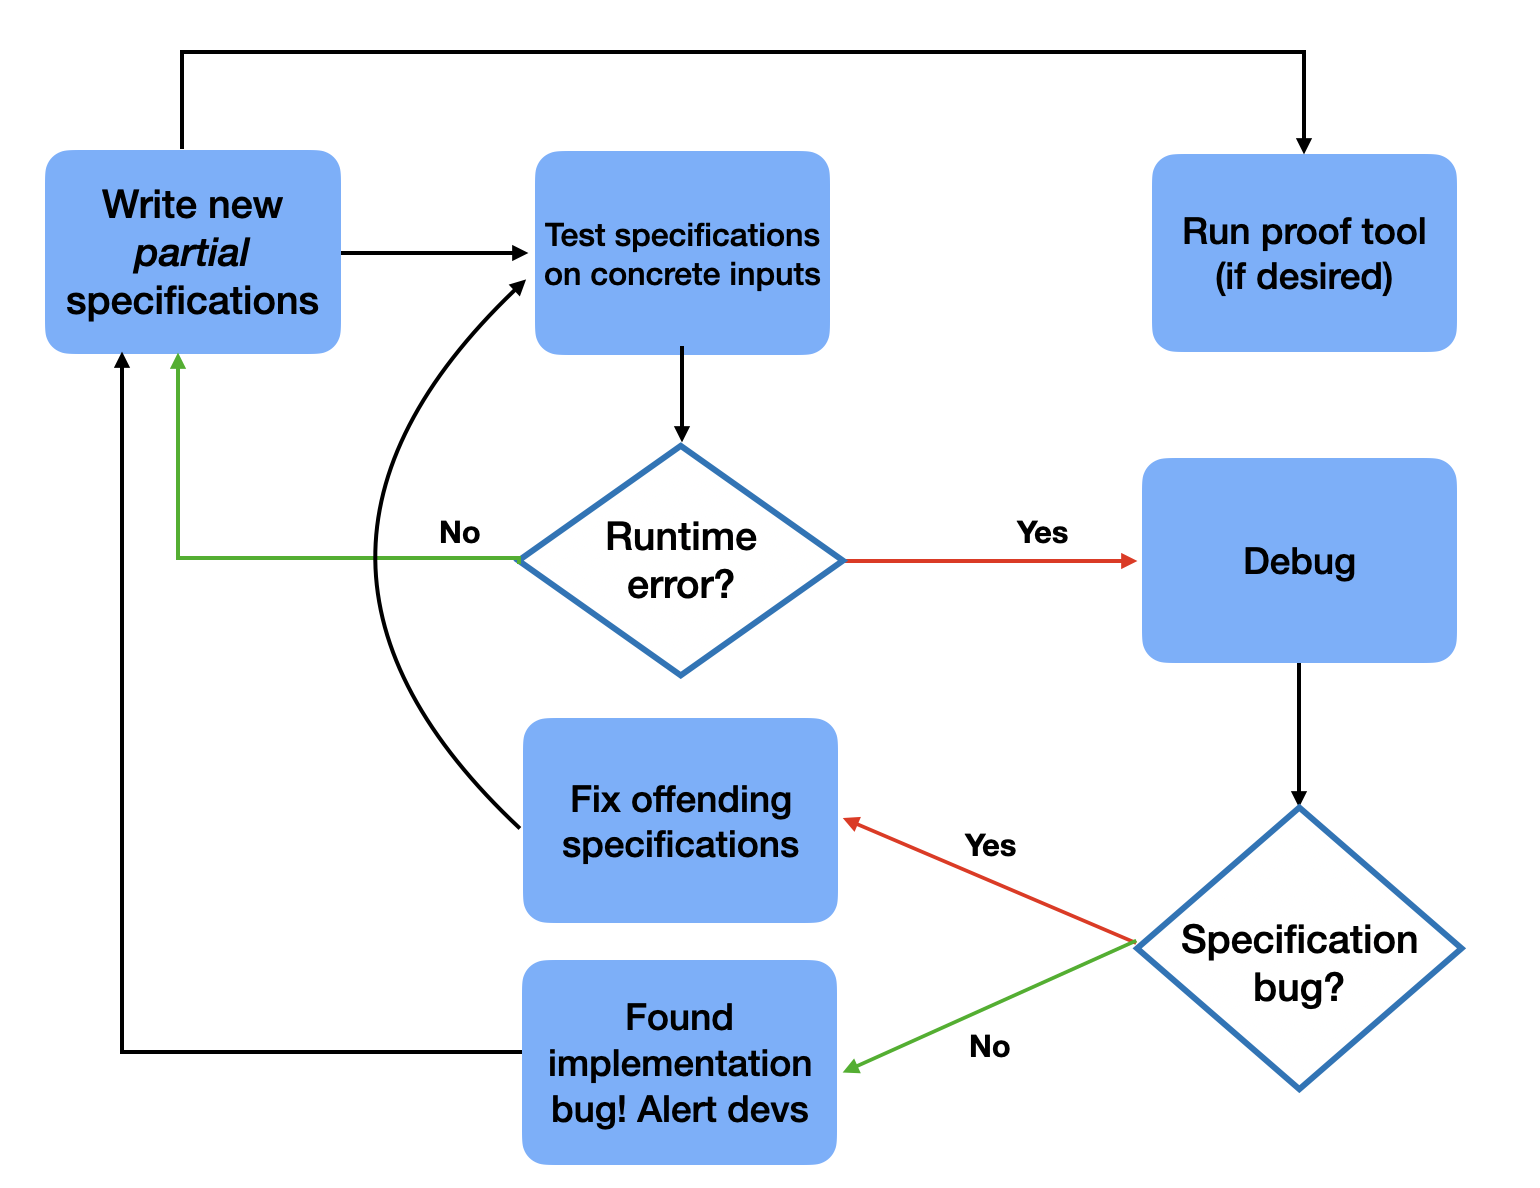
\includegraphics{assets/code-spec-test-debug-prove.png}
%   }
%   \caption{Code-Specify-Test-Debug-Prove. \textbf{TODO}: redo, this is just copied from my Keynote}
% \end{figure}

% Code-Specify-Test-Debug-Prove. Generic here; can make concrete later with CN toolchain for C code.

% Include diagram from Keynote slides. Make diagram more generic; our work has been without the Code part of the cycle, so I made diagram specific to the retroactive case, but it needs to be more general. (Diagram currently starts with ``Write partial specs'' which assumes a pre-existing codebase)

% \section{Testing separation-logic specifications}

% Focus now on systems setting. Motivate why reliability of systems software so important (bug propagating upward, affecting all software running on top of it), and say most systems software is written in C. Look at Kayvan thesis related work briefly?

% \subsection{Separation logic}

% History:

% Hoare logic not good for reasoning about aliasing pointers. Number of inequalities blows up. Motivated creation of separation logic by Reynolds and O'Hearn. $p \mapsto v$, $A \ast B$, frame rule. See LFCS/Birmingham slides. Active research area, lots of research in it today. Link back to systems setting -- these operators make heap memory reasoning compositional which is great when reasoning about programs written in e.g. C or Rust.

% \subsection{Executing separation logic}

% Comment on technical difficulty of executing $\ast$ operator and give example of how it blows up. Backtracking, arbitrary quantification over pointers, etc.

\section{Thesis statement}

NK 29/04: a useful thing to write down first, even if it won't be understood by anyone else without the context that comes before this.

\section{Thesis outline}
\section{Publications} 
(incl. publications, collaborators -- maybe a few sentences, doesn't need its own subsection)

PS 29/04: Thesis outline and publications might become a single section. Plus discussion of exactly which bits I did.





\chapter{Related work}

PS 29/04: Not ``just a related work'' to get out of the way. Need to link with other areas and compare and contrast against them in various ways. PS says to try to avoid entering the rabbit hole too much before first writing some more (e.g. intro first). But need to do that a little bit to understand the shape of the related work and what I actually want to say! 

See first-year report as a starting point.

\begin{enumerate}
  \item Executable specifications
  \begin{enumerate}
    \item Hoare Logic runtime specification checking (incl. E-ACSL) - no ownership
    \item Linear logic runtime checking - Limin Jia PhD thesis - not SL
    \item Contract checking literature
    \item SLICK (Java runtime SL checking) - not C
  \end{enumerate}
  \item C separation-logic verification tooling (similar tools but specs not executable or not applicable to real-world C code) -- e.g. RefinedC, Gillian. See CN and Fulminate papers' related work sections
  \item Gradual verification -- e.g. Gradual C0
\end{enumerate}


\chapter{A motivating example}

% Goal: Reader should just be able to look at this chapter and know how Fulminate works at a high level.

% In this chapter, we consider a typical singly-linked list implemented in C and one of its operations, demonstrating how one can use Fulminate to gradually specify and verify the latter. 

In this chapter, we take a look at how Fulminate works at a high level, using a classic separation logic example of a singly-linked list, with the list and its operations implemented in C and its specifications written using CN. TODO: rewrite this para once chapter done

% {\color{violet}
% New section outline (?):

% \begin{itemize}
%   \item Start with the C you want to specify/test
%   \item Then go to separation-logic predicate you'd like to write
%   \item Then show CN
%   \item Then the rest, executing in Fulm, writing spec in CN and testing in Fulm. Is that where we show the Fulm output? Need to show the pre and postcondition code and where injection is happening, but also the actual \texttt{IntList} predicate in C and how it just easily translates to that
% \end{itemize}
% }

% \section{A singly linked-list and its operations, in C}

% \begin{center}
% \lstinputlisting[language=CNC]{code_snippets/append.c}
% \end{center}

% TODO: explain linked-list struct and imperative (non-recursive) implementation -- idiomatic C. Segue into needing \texttt{IntList} predicate to specify this.

\section{A singly-linked list, in C}\label{sec:linked-list-in-c}

Consider the following struct definition in C, representing a singly-linked list: 

\begin{center}
\lstinputlisting[language=C, numbers=none]{code_snippets/linked_list_def.h}
\end{center}

A \texttt{struct node} has, by this definition, a fixed-width integer value associated with it and a pointer to the next node in the list, also of type \texttt{struct node}. This definition can be unfolded recursively via the \texttt{next} member until this pointer is null, meaning the end of the linked list has been reached.

For example, the following C code uses this definition to create a linked list with elements 1, 2 and 3, starting at \texttt{i1}:

\begin{center}
\lstinputlisting[language=C, numbers=none, firstline=3]{code_snippets/linked_list_concrete.c}
\end{center}

This construction is done in reverse order, starting at the last element, such that the list can be ``chained'' together in memory as it is being constructed via the \texttt{next} pointers.

Now consider the following \texttt{list\_append} operation on two such singly-linked lists, also implemented in C:

\begin{center}
\lstinputlisting[language=C, firstline=3]{code_snippets/append.c}
\end{center}

This takes two arguments of type \texttt{struct node}, \texttt{xs} and \texttt{ys}. If \texttt{xs} is the null pointer, the function returns \texttt{ys}; otherwise, it traverses \texttt{xs} through to its last element, and sets the \texttt{next} pointer of that element to be \texttt{ys}.

To get higher assurance that this code behaves the way we expect it to, we might like to test it, or verify it, or both; this might naturally lead us towards wanting to write a specification for this function. 

\section{Specification desiderata}

Ideally, we would like our specification for \texttt{list\_append} to:

\begin{enumerate}
  \item Describe certain \emph{functional} properties -- e.g.~what the integer elements of the returned, concatenated list are in relation to the elements of the input lists.
  \item Describe \emph{ownership} properties, since we are dealing with low-level C code that involves explicit pointers and their fine-grained manipulation -- here, we care especially about the structure of the lists in memory on entry to and exit from the function.
  \item Be \emph{executable} for the purpose of testing, but also usable for verification if desired. The executability of the specification is important not just for standalone testing of the C function, but also for being able to test the specification itself as we write it in an incremental fashion.
\end{enumerate}

The first goal is achievable using Hoare logic, but the second is not -- for tractable ownership reasoning, separation logic is needed. Thus, for the third goal to also hold, the separation-logic specification we write for \texttt{list\_append} must be executable -- and this is not obviously possible on first glance, as we explain in the next section. 

\section{Executing separation-logic specifications}

\subsection{Classical separation logic is not executable}

To understand why this is the case, consider the following separation-logic predicate \texttt{IntList}, which formally describes a singly-linked list of the form we saw in Section~\ref{sec:linked-list-in-c}:

\begin{figure}[h]
  \vspace{-0.8em}
  \begin{align*}
  \text{IntList}(p, \alpha) =\, &(p = \text{NULL} \land \alpha = \lbrack\rbrack)\\
  &\lor (\exists{hd}, q, {tl}.\,p \mapsto ({hd}, q) \ast \text{IntList}(q, {tl}) \land \alpha = {hd} :: {tl})
  \end{align*}
  \vspace{-2em}
\end{figure}

This predicate takes two inputs: a pointer $p$ that is either the null pointer, or points to the head of some linked list in memory, and a mathematical list $\alpha$, an abstract representation of the linked list's values. In the case where $p$ is not null, this predicate asserts ownership over the entire list one node at a time, via the points-to assertion and the recursive call to \texttt{IntList}.

What would it mean to execute this predicate as part of some function-level specification? Rather than proving that these properties hold statically for any arbitrary $p$ and $\alpha$, we want to check for some concrete values of $p$ and $\alpha$, and the corresponding concrete heap, that we can assert the correct ownership over all nodes of the linked list, and that all of the expected logical properties hold. 

However, this predicate does not look particularly executable on first glance.

\begin{enumerate}
  \item There is a disjunction, which might require backtracking depending on whether $p$ is the null-pointer or not. In this case, this is detectable early in the execution of the first disjunct, but for arbitrary disjunction, this is not guaranteed.
  \item The second disjunct contains existential quantification over ${hd}$, $q$ and ${tl}$, which might require searching for values.
  \item There is an instance of the separating conjunction $\ast$, which requires searching for disjoint splittings of the heap -- this blows up quickly with the size of the heap, with a heap of size $n$ requiring $2^n$ possible splittings to be searched.
\end{enumerate}

Thus, executing a classical separation-logic specification is, in the general case, computationally infeasible. The next section describes how carefully restricting the logic can eliminate these barriers to executability.


\begin{figure}[h]
  \begin{center}
    \begin{minipage}[t]{.28\textwidth}
      \vspace{-6.2em}
      \lstset{
      numbers=left,
      firstnumber=1,
      numberfirstline=true
      }
      % \vspace{0.2em}
      \scalebox{0.9}{\lstinputlisting[language=CNC, lastline=12]{code_snippets/intlist.cn.c}}
    \end{minipage}
    %
    %
    \hspace*{8.5\baselineskip}
    \begin{minipage}[t]{.28\textwidth}
      \lstset{
      numbers=left,
      firstnumber=13,
      numberfirstline=true
      }
      \scalebox{0.9}{\lstinputlisting[language=CNC,firstline=13]{code_snippets/intlist.cn.c}}
    \end{minipage}
    % \vspace*{0.8\baselineskip}
  \end{center}
  \vspace*{-4mm}
  \caption{The \texttt{IntList} predicate, written in the CN specification language. The CN definitions are enclosed in magic comments {\color{commentcolour}$/*@ \ldots @*/$} (lines 1-12, 18-23). The \texttt{IntList} predicate definition relies on the the C \texttt{struct node} definition (lines 13-16), which is the same as the one introduced in Section~\ref{sec:linked-list-in-c}.}
  \label{fig:intlist-cn}
\end{figure}

\subsection{CN separation logic \underline{is} executable!}

Now consider the same \texttt{IntList} predicate, written in the CN specification language, as shown in Fig.~\ref{fig:intlist-cn}. The CN predicate definition is on the left hand side, with auxilliary C and CN definitions on the right. The CN definitions are enclosed in ``magic comments'' ({\color{commentcolour}$/*@ \ldots @*/$}), such that they can be parsed and desugared by the CN toolchain and treated like usual comments by any C compiler such as clang or gcc. 

\TODO{rename node variable to something else? it's confusing for the variable and the struct tag to have the same name}

The \texttt{IntList} predicate signature on line 2 states that the predicate takes a single argument $p$ of generic pointer type, and returns a \texttt{datatype seq}, which is defined on lines 19-22 as a CN datatype with two constructors, \texttt{Nil} and \texttt{Cons}. The \texttt{rec} keyword indicates that the predicate is recursive. The predicate first checks whether the pointer $p$ is null, returning the \texttt{Nil} constructor if that is the case (lines 3-5). Otherwise, it extracts the value stored at $p$ using CN's builtin \texttt{Owned} predicate, storing it in a new variable called \texttt{node} (line 7). (Note the angle brackets $\langle\ldots\rangle$, which denote the expected C type of $p$'s value -- here, this has type \texttt{struct node}, defined on lines 13-16 as a usual C singly-linked list with some \texttt{head} value and a \texttt{next} pointer to the rest of the list.) After that, \texttt{IntList} is called recursively on the \texttt{next} pointer of $p$'s value, with the associated mathematical list datatype stored in a new variable \texttt{tl} (line 8). Finally, the 32-bit integer \texttt{head} member of \texttt{node} (which we recall has type \texttt{struct node}) and the mathematical abstraction of the rest of the list are composed under the \texttt{Cons} constructor and returned (line 9).  

\TODO{Following para might need to be rejigged slightly to improve flow}

This CN predicate differs from its classical analogue in several ways: it takes the pointer $p$ as its only argument rather than both the pointer and its mathematical list representation $\alpha$; it has an if-else statement that checks whether $p$ is NULL instead of using logical disjunction to account for either case; and it constructs and returns the mathematical list $\alpha$ as a CN datatype. Crucially, points-to assertions are written in CN using its builtin \texttt{Owned} predicate: $p \mapsto v$ is written as $\texttt{take}\,\,v = \texttt{Owned}\langle\textit{ctype}\rangle(p)$, with CN's syntax restricting $v$ to be an output parameter here rather than an input that could be arbitrarily quantified over. The $\ast$ operator is encoded by CN's semicolons, ensuring each assertion holds for disjoint parts of the heap.

This version of the \texttt{IntList} predicate \emph{looks} executable, and it turns out that it is. CN's restrictive syntax, originally designed to make the CN proof tool's automation more predictable, is exactly what enables it to be executed -- and this is what Fulminate sets out to do.

\subsection{Fulminate executes CN specifications}

Fulminate is a tool that takes a C file with CN annotations, and transforms these into C runtime checks, producing an instrumented C file with executable separation-logic specification checks. For example, Fulminate takes the CN \texttt{IntList} example in Fig.~\ref{fig:intlist-cn} as input and produces the C code in Figs~\ref{fig:intlist-fulm-datatype-defs} and \ref{fig:intlist-fulm}.

\begin{figure}[h]
  \begin{center}
    \begin{minipage}[t]{.18\textwidth}
      % \vspace{-6.2em}
      \lstset{
      numbers=left,
      firstnumber=1,
      numberfirstline=true
      }
      \vspace{0.2em}
      \lstinputlisting[language=CNC, firstline=5, lastline=20]{code_snippets/intlist.cn.exec.c}
    \end{minipage}
    %
    %
    \hspace*{8.5\baselineskip}
    \begin{minipage}[t]{.3\textwidth}
      \lstset{
      numbers=left,
      firstnumber=17,
      numberfirstline=true
      }
      \lstinputlisting[language=CNC,firstline=22, lastline=38]{code_snippets/intlist.cn.exec.c}
    \end{minipage}
    % \vspace*{0.8\baselineskip}
  \end{center}
  \vspace*{-4mm}
  \caption{Top-level type definitions produced by Fulminate when applied to CN \texttt{IntList} example.}
  \label{fig:intlist-fulm-datatype-defs}
\end{figure}

\begin{figure}[h!]
  \begin{center}
  \lstset{
    numbers=left,
    firstnumber=35,
    numberfirstline=true
  }
  \lstinputlisting[language=C, firstline=40, lastline=59, breaklines]{code_snippets/intlist.cn.exec.c}
  \end{center}
  \caption{Fulminate-translated C function definition of the CN \texttt{IntList} predicate.}
  \label{fig:intlist-fulm}
\end{figure}




% \section{Executing \texttt{IntList}}

\section{Writing and testing a specification for \texttt{list\_append}, using Fulminate}

We can now consider the following C implementation of a singly-linked list and its append operation, specified in CN using the \texttt{IntList} predicate we just defined:

\TODO{fix C spacing}

\TODO{Either add append function implementation and Seq datatype or note their absence explicitly}

\TODO{Check this new imperative implementation actually works with CN and Fulminate, with same spec}

\begin{figure}
  \begin{center}
  \lstinputlisting[language=CNC]{code_snippets/append.cn.c}
  \end{center}
\end{figure}





% Do example with partial specifications. Include error messages, debugging with \texttt{lldb}, etc

% \section{The CN separation-logic specification language}

% Cover $p \mapsto v$ and \texttt{Owned}
% IntList example (should be in above spec example) and side-by-side comparison between standard SL formulae and CN representation. 


% \section{Writing partial CN specifications using Fulminate}

% Assuming we have a pre-existing C function to specify in this case.

% Small spec example, using IntList. Explain CN semicolon is $\ast$. 

% Say Fulminate takes CN+C files, gives C file with checks in the expected places. Fulminate tracks ownership of stack-local and heap addresses; instruments access checks to ensure ownership of an address has been asserted properly before it is read from or written to.

% Show Fulminate runtime ownership error from partial spec, debug and fix up spec, run again.




\chapter{Design goals \& choices}

TODO: Expand
TODO: Take goals from first-year report/why testing? slide from keynote. And, remember that real-world software engineers are more likely to be familiar with testing and writing partial inline assertions than ``fancy'' mathematical/separation-logic/formal-methods constructs, proof, etc.

\newcommand{\myparagraph}[1]{\paragraph{#1}}


{\color{red}
The above observation is simple, especially in hindsight, but going from that to a practical system for runtime testing of CN assertions for actual C code requires one to consider many design and implementation questions. 
%
We begin with some high-level goals and how they have determined our design.


\myparagraph{Runtime testing on concrete executions}
Fulminate supports runtime testing of CN assertions, covering both their ownership and pure-value aspects,
in concrete execution of the underlying C program.
%
Like other runtime testing approaches, it is thus testing whether pre- and post-conditions hold of the concrete states reached at those program points within a complete execution, not whether pre-conditions imply post-conditions.

\myparagraph{Flexible usage models for a shallow on-ramp to higher assurance}
Fulminate aims at a very lightweight user experience, providing a gentle on-ramp to higher assurance in a variety of testing and testing+proof workflows.
Conventional developers, who are not verification experts, might start by writing partial CN specifications
-- initially not much more than C \lstinline{assert}s --
and get immediate benefits from them by quickly detecting errors in CN testing, without any proof whatsoever. They could then gradually add richer ownership and functional-correctness properties.
In higher-assurance contexts, verification experts might extend these and write more specifications for proof, in exactly the same CN specification language, and use Fulminate to
quickly debug both their specifications and their code by testing them, interleaved with using CN refinement-type proof to verify them. 

\myparagraph{Testing of (a substantial fragment of) actual C}
Fulminate supports a substantial fragment of actual C, rather than an idealised C-like language (though there are a number of features that are not yet supported, as we describe in \S\ref{sec:conc}).
To this end, it uses the front-end of the Cerberus C semantics by Memarian et al.~\cite{CerberusPLDI16,cerberus-popl2019,UCAM-CL-TR-981} to parse, typecheck, and desugar C source files, as does CN.
To inject the translations of CN specifications into the C code, we have developed new machinery as a part of Cerberus.



\myparagraph{Testing using conventional build processes and tools, and with arbitrary existing test harnesses and tests}
Like systems from
Anna~\cite{DBLP:journals/software/LuckhamH85} to the Frama-C E-ACSL~\cite{DBLP:conf/sac/DelahayeKS13,DBLP:books/hal/Signoles18,DBLP:conf/issta/Signoles21}, Fulminate is structured as an annotated-C to C source-to-source translation, which adds instrumentation to check the CN specifications.  The result of this translation can be built with a conventional C compiler, just like the original C source. The instrumented binary can then be executed in the same way as the original program, in whatever test harness and on whatever test suite the developers normally use.
%
It is an on-line checker, obviating the need for logging that an off-line checker would have.  Fulminate checking (optionally) %\TODO{have to actually implement the 'optionally`}
 involves checking every memory access, so logs would quickly become very large. 


\myparagraph{Design for usability: error reporting}
Design for usability also makes it essential to give good error reports on runtime test failures,
including e.g.\ both the C source location and CN predicate-definition source location
on runtime ownership and other failures.  
We plan also to include optional ghost state to support reporting of which CN predicates own which parts of the heap, and thus which are involved in ownership errors.
%    - design for good error reports (eg recording real source locations, and metadata for 
%      which predicates).
Even highly expert kernel developers may not have the ownership patterns of their code explicitly in mind, as they currently have no way to write them down, beyond prose comments, and no way to test or verify them.  CN specifications and such feedback from testing may help develop a solid intuition and understanding of this.
%
%strengthen user intuition for ownership
%         (even very strong devs may not have ownership very expliitly in their heads - 
%          they have no way to write it down or test it)

\myparagraph{Design for usability: debugging dynamic failures}
Design for debuggability leads us to build a translation that closely follows the structure of the source program, preserving its layout and comments, and with readable C for the instrumentation. This means one can, for example, sensibly use gdb or lldb on the generated code -- including examination of the abstract states computed by CN predicates, and the reasons why CN assertions fail.

%\TODOPS{can we use nice CN-generated printers from the debugger?}

\myparagraph{Minimal dependencies for bare-metal execution}
One of our intended targets is systems code that runs in restricted execution environments, including hypervisor code such as Google's Android pKVM hypervisor~\cite{pKVM-linux-talk}, which runs as an isolated component at Arm-A Exception Level (EL) 2, above the Android kernel at EL1 and user code at EL0. 
Such code has to work in a very limited context, without the C standard library or most operating-system services. Fulminate has not yet been demonstrated running at EL2,
%\TODOPS{can we?},
but this goal leads us to make the generated instrumentation essentially bare-metal C, without runtime dependencies.


\myparagraph{Performance}
%
Runtime testing is intrinsically expensive compared with uninstrumented execution, and runtime testing of separation logic predicates and ownership has to walk the relevant part of the heap, and check and/or update the corresponding ghost state, whenever such a specification is reached.  
%
Compared with sanitizers, for example, Fulminate is checking much richer properties, and one should expect it to have substantially more performance cost.
%
However, Fulminate targets relatively small bodies of critical C code. 
Our working hypothesis is that, for such code operating over relatively small datastructures, even a relatively naive implementation is fast enough to be useful, and to explore how it behaves in practice -- so long as it is on-line and translates to reasonable C, as described above.   There are many potential optimisations, and the underlying scheme would support sampling -- checking only a random subset of function executions -- but we do not explore them in this paper. 

% this is really future work, but maybe it's nice to put here to ameliorate the performance downside?
\myparagraph{Test generation}
Fulminate does not itself do test-case \emph{generation}, but it should work well with property-based testing: if one can automatically synthesise unit test cases, benefitting from CN ownership specifications for function preconditions, then one will be able to test the rich CN properties in unit-test executions, making performance much less critical.  Fulminate may also work well with fuzzing, guiding fuzzing with rich-specification failures.
}

\myparagraph{Bridging testing and proof gap}
Bridging gap between testing and proof/inferring proof hints/underapprox+overapprox/gradual story


\chapter{Formalisation}

Fulminate paper, link to Dhruv's supplementary material and credit him (+ Hiro if including partial spec formalisation).

TODO: Ask Hiro about partial spec formalisation

\chapter{Implementation}

\section{Architecture}

\begin{figure}
% \begin{verbatim}
%          C program + CN annotations -------------------------------------------
%                 |                                                             |
%          Cerberus front-end                                                   |
%          (parsing, desugaring, and C type inference/checking)                 |
%                 |                                                             |
%          Typed Ail  ----------------------------------------------------|     |
%                 |                                                       |     |
%           Cerberus elaboration                                          |     |
%        /                          \                                     |     |
%     Core                              MuCore               -----        |     |
%        |                                |                       \       |     |
% Core operational semantics        CN proof tooling                ->Fulminate translation
%        |                         (refinement type inf)                  |
%        |                                |                               |
%    executions                      yes/no                               C
%                                                                         |
%                                                                     gcc/clang
%                                                                         |
%                                                                       executions with failures
% \end{verbatim}


\tikzset{%
  >={Latex[width=2mm,length=2mm]},
  % Specifications for style of nodes:
            artifact/.style = {
                           minimum width=1cm, minimum height=0.3cm,
                           text centered, font=\rmfamily\small},
            base/.style = {rectangle, rounded corners, %draw=black,
                           minimum width=1cm, minimum height=0.3cm,
                           text centered, font=\rmfamily\small},
  activityStarts/.style = {base, fill=blue!30},
       startstop/.style = {base, fill=red!30},
    activityRuns/.style = {base, fill=green!30},
         process/.style = {base, minimum width=1cm, fill=orange!15,
                           font=\rmfamily\small},
}

\begin{tikzpicture}[node distance=1.2cm,
    every node/.style={fill=white, font=\rmfamily\small}, align=center]

  \node (CandCN)             [artifact]              {C program + CN annotations};
  \node (frontend)           [process, below of=CandCN] {Cerberus front-end\\\footnotesize parsing, desugaring, C type inference/checking};
  \node (TypedAil)           [artifact, below of=frontend]  {Typed Ail\\\footnotesize Typed C abstract syntax};
  \node (elab)               [process, below of=TypedAil]   {Cerberus elaboration};

  \node (Core)               [artifact, below of=elab, xshift=-2.2cm, text=black!30] {Cerberus Core of C};
  \node (CoreOpsem)          [process, below of=Core, text=black!30]           {Core operational semantics};
  \node (CoreEx)             [artifact, below of=CoreOpsem, text=black!30]     {Core executions};

  \node (MuCore)             [artifact, below of=elab, xshift=2.2cm] {MuCore of C + MuCore of CN};
  \node (CNproof)            [process, below of=MuCore]          {CN proof tooling\\\footnotesize refinement type inference+SMT};
  \node (verif)              [artifact, below of=CNproof]     {CN verification yes/no};


  \node (Fulm)             [process, below of=elab, xshift=6.6cm, yshift=-1.2cm] {Fulminate\\\footnotesize C+CN to C translation};
  \node (C)                [artifact, below of=Fulm]          {generated C};
  \node (gcc)              [process, below of=C]            {gcc/clang};
  \node (Cexec)            [artifact, below of=gcc]          {conventional binary executions with \\CN specification failure detection};

  \node (gccplain)              [process, below of=elab, xshift=-6.6cm, yshift=-3.6cm]   {gcc/clang};
  \node (Cexecplain)            [artifact, below of=gccplain]          {conventional\\binary executions};


  \draw[->] (CandCN) -- (frontend);
  \draw[->] (frontend) -- (TypedAil);
  \draw[->] (TypedAil) -- (elab);

  \draw[->, black!30] (elab) to  (Core);
  \draw[->, black!30] (Core) -- (CoreOpsem);
  \draw[->, black!30] (CoreOpsem) -- (CoreEx);

  \draw[->] (elab) -- (MuCore);
  \draw[->] (MuCore) -- (CNproof);
  \draw[->] (CNproof) -- (verif);

  \draw[->] (MuCore.east) to [bend left=5] (Fulm);
  \draw[->] (Fulm) -- (C);
  \draw[->] (C) -- (gcc);
  \draw[->] (gcc) -- (Cexec);

  \draw[->] (CandCN) to [bend left=38] (Fulm);
  \draw[->] (TypedAil) to [bend left=10] (Fulm);

  \draw[->] (CandCN.south west) to [bend right=38] (gccplain);
  \draw[->] (gccplain) -- (Cexecplain);



\end{tikzpicture}
\caption{Fulminate architecture (\textbf{TODO}: fix overlapping boxes)}\label{fig:fulm}
\end{figure}

\begin{enumerate}
  \item architecture diagram (credit PS)
  \item CN+C file $\rightarrow$ Shared CN+Cerberus frontend $\rightarrow$ Typed Ail + Mucore $\rightarrow$ Ail to be injected back $\rightarrow$ Strings to be injected back $\rightarrow$ C file with instrumentation
  \begin{enumerate}
    \item CN has two (?) ASTs -- external untyped AST and internal typed AST. We choose the latter as we need to know the basetypes in Fulminate (explain why)
  \end{enumerate}
  \item discuss alternative -- taking Typed Ail program and injecting Ail statements into that directly, and then pretty-printing the whole Ail program. Wouldn't work with existing Ail pretty-printer, which doesn't print valid C in general, and also messes with the shape of the source in unclear ways (enumerate some things Ail abstracts away, e.g. enums), which makes debugging with lldb/knowing which parts are Fulminate and which were already in the source more unclear
\end{enumerate}

\section{Top-level translation machinery}\label{sec:top-level-translation}

Some covered in motivating example, probably.

\subsection{Preconditions}
\subsection{Postconditions}
\subsection{Loop invariants}
paper text, including from appendix


\section{Translation of pure expressions}

Link to \S\ref{sec:cn-index-terms}

Describe destination passing~\cite{destinationPassing} for translating from CN (expression language) to C (statement language).


\textbf{TODO}: Double-check the following list covers all index terms in appendix.

\subsection{Constants}
\subsection{Symbols} including special handling of globals in \texttt{accesses} clauses, using \texttt{is\_sym\_obj\_address}
\subsection{Unary and binary operators}
\subsection{If-then-else}
\subsection{Iterated logical conjunction}
\subsection{Structs}
Structs in CN can only refer to C structs that have already been defined in source (???) check
\subsection{Records}
\subsection{Datatypes}
\texttt{Constructor} and pattern matching - matrix algorithm~\cite{matrixAlgorithm}

\subsection{Member shift and array shift}
\subsection{Sizeof and offsetof}
\subsection{Maps}
\subsection{Lemma (and function?) application}
\subsection{Let expressions}
\subsection{Casts}

\subsection{Unsupported expressions}

\texttt{AllocID} stuff all for VIP


\section{Resources and ownership}

\subsection{Overview}

Global ownership ghost state mapping bytes of memory to ``their'' (better phrasing) stack depth. Diagram of ghost state. Intuition for what it means and what types of errors we can catch via this mapping. 

Mention that all memory accesses (Ail program analysed to instrument all loads and stores) are wrapped with calls to \texttt{CN\_LOAD} and \texttt{CN\_STORE} macros (and explain what they do). Enumerate and mention postfix macro too, all in \texttt{utils} library


\subsection{\texttt{Owned}}
Tie back to scheme described in overview at start of section. Works differently depending on whether call to \texttt{Owned} in precondition, postcondition, or loop (see \S\ref{sec:top-level-translation})
\subsection{Iterated separating conjunction}

\begin{enumerate}
  \item only works for bounded conjunctions
  \item mention recent optimisations for asserting ownership in a single call for contiguous memory regions and not creating maps when never used. Can do more and make it cleverer...
\end{enumerate}


\subsection{Stack-allocated locals}

Mapping their addresses to ghost state. C control flow support: \texttt{return}, \texttt{goto}, \texttt{break}, \texttt{continue}. C memory access instrumentation works with this scheme.

\subsection{Globals}

via \texttt{accesses} and calling back to special case in translation of \texttt{Sym}

\section{Translation of top-level constructs}

\subsection{Functions}
\subsection{Predicates}
\subsection{Datatypes}
\subsection{Lemmas}
\subsection{Ghost arguments}


\section{The C runtime library}

Anything that isn't source-dependent, we have handwritten into the C runtime library.

\subsection{Ghost types}

Weird macros galore.

\subsection{Allocator}

\begin{enumerate}
  \item Initially giant static array
  \item Then bump allocator and free list allocator
  \item Now bump allocator for specifications with known lifetimes (e.g. function-level spec's lifetime is until end of function execution/executable postcondition, loop invariant's lifetime is until the end of the single iteration of the loop thereafter)
\end{enumerate}

\section{Dealing with the C}

\begin{enumerate}
  \item Having to preprocess
  \item What it was before: outputting several files, including \texttt{source.exec.c}, \texttt{cn.c}, \texttt{cn.h} etc to keep defs nice and tidy, but having to preprocess inside Fulminate meant we had to change to output a single file
  \item Struct craziness, which I believe went away as a nice offshoot of having to preprocess and output a single giant file
  \item C runtime library needing to be so baremetal (or in prev. section)
\end{enumerate}

\section{Usability}

\subsection{Error messages}

\textbf{TODO}: fix. Two types: source location information and instrumented file location.

\subsection{Integration with existing debuggers}

\texttt{gdb}, \texttt{lldb}. Look at what HK wrote in PLDI paper 

\section{Partial specifications}

Why do we need them? Usability reasons - motivate. Explain using problems experienced when Fulminate didn't support these.

\begin{enumerate}
  \item Partial function-level specs
  \item Fragmentary specs
  \item Wildcard ownership
\end{enumerate}




\chapter{Case studies}

PS 29/04: Calling this section ``Evaluation'' is kind of underselling the importance of this chapter.

\begin{itemize}
  \item Tutorial examples (CN, Verifast, incremental stack example)
  \item pKVM
  \begin{itemize}
    \item what is pKVM
    \item buddy allocator
    \item hyp allocator
  \end{itemize}
\end{itemize}



% \section{Applying Code-Specify-Test-Debug-Prove}

% \section{Performance}

% copy-paste from PLDI '26 paper

% \section{Bugs}

% Specification bugs; Hiro's experience section from PLDI paper.

% \section{Usability}

% Say upfront we don't have anything sophisticated like user studies. (check status of DARPA ones)

\begin{itemize}
  \item integration with LLDB
  \item error messages (TODO: improve + fix)
\end{itemize}

\chapter{Conclusion}

speculate on future directions (e.g. concurrency, VIP)

\section{Future work}

\bibliographystyle{plainnat}
\bibliography{thesis}




%%%%%%%%%%%%%%%%%%%%%%%%%%%%%%%%%%%%%%%%%%%%%%%%%%%%%%%%%%%%%%%%%%%%%%%%%%%%%%%%
%% Appendix:
%%

\appendix

\chapter{CN types in OCaml}

\section{CN index terms}\label{sec:cn-index-terms}

\begin{minted}[breaklines]{ocaml}
(* over integers and reals *)
type 'bt term =
  | Const of const
  | Sym of Sym.t
  | Unop of unop * 'bt annot
  | Binop of binop * 'bt annot * 'bt annot
  | ITE of 'bt annot * 'bt annot * 'bt annot
  | EachI of (int * (Sym.t * BaseTypes.t) * int) * 'bt annot
  (* add Z3's Distinct for separation facts *)
  | Tuple of 'bt annot list
  | NthTuple of int * 'bt annot
  | Struct of Sym.t * (Id.t * 'bt annot) list
  | StructMember of 'bt annot * Id.t
  | StructUpdate of ('bt annot * Id.t) * 'bt annot
  | Record of (Id.t * 'bt annot) list
  | RecordMember of 'bt annot * Id.t
  | RecordUpdate of ('bt annot * Id.t) * 'bt annot (* this is currently unused *)
  | Constructor of Sym.t * (Id.t * 'bt annot) list
  | MemberShift of 'bt annot * Sym.t * Id.t
  | ArrayShift of
      { base : 'bt annot;
        ct : Sctypes.t;
        index : 'bt annot
      }
  | CopyAllocId of
      { addr : 'bt annot;
        loc : 'bt annot
      }
  | HasAllocId of 'bt annot
  | SizeOf of Sctypes.t
  | OffsetOf of Sym.t * Id.t
  | Nil of BaseTypes.t
  | Cons of 'bt annot * 'bt annot
  | Head of 'bt annot
  | Tail of 'bt annot
  | Representable of Sctypes.t * 'bt annot
  | Good of Sctypes.t * 'bt annot
  | Aligned of
      { t : 'bt annot;
        align : 'bt annot
      }
  | WrapI of Sctypes.IntegerTypes.t * 'bt annot
  | MapConst of BaseTypes.t * 'bt annot
  | MapSet of 'bt annot * 'bt annot * 'bt annot
  | MapGet of 'bt annot * 'bt annot
  | MapDef of (Sym.t * BaseTypes.t) * 'bt annot
  | Apply of Sym.t * 'bt annot list
  | Let of (Sym.t * 'bt annot) * 'bt annot
  | Match of 'bt annot * ('bt pattern * 'bt annot) list
  | Cast of BaseTypes.t * 'bt annot
  | CN_None of BaseTypes.t
  | CN_Some of 'bt annot
  | IsSome of 'bt annot
  | GetOpt of 'bt annot

and 'bt annot =
  | IT of 'bt term * 'bt * (Locations.t[@equal fun _ _ -> true] [@compare fun _ _ -> 0])
[@@deriving eq, ord, map]
\end{minted}



%%%%%%%%%%%%%%%%%%%%%%%%%%%%%%%%%%%%%%%%%%%%%%%%%%%%%%%%%%%%%%%%%%%%%%%%%%%%%%%%
%% Index:
%%
\printthesisindex

\end{document}
